%%%%%%%%%%%%%%%%%%%%%%%%%%%%%%%%%%%%%%%%%%%%%%%%%%%%%%%%%%%%
% 1.11 REPRESENTATION THEORY
% The Composition of Advanced Mathematics
%%%%%%%%%%%%%%%%%%%%%%%%%%%%%%%%%%%%%%%%%%%%%%%%%%%%%%%%%%%%

\section{Representation Theory}
\label{sec:representation-theory}

\prerequisite{
Linear algebra from \cref{sec:linear-algebra}, group theory from
\cref{sec:group-theory}, module theory from \cref{sec:module-theory}, and
noncommutative algebra from \cref{sec:noncommutative-algebra}.
}

\learningobjectives{
By the end of this section, the reader should be able to:
\begin{itemize}
    \item explain the purpose of representing abstract algebraic objects by linear transformations;
    \item define a group representation and its degree;
    \item distinguish faithful, trivial, permutation, regular, and irreducible representations;
    \item convert between linear transformations and matrix representations;
    \item determine invariant subspaces and subrepresentations;
    \item define reducible and irreducible representations;
    \item construct direct sums of representations;
    \item define equivalent representations and intertwining maps;
    \item explain representations as modules over group algebras;
    \item state and apply Maschke's theorem;
    \item define characters and compute basic character values;
    \item use character inner products to test irreducibility and equivalence;
    \item understand the basic structure of character tables;
    \item recognize the regular representation and its decomposition;
    \item define tensor-product, dual, and quotient representations;
    \item explain Schur's lemma and its structural significance;
    \item connect representation theory with symmetry, geometry, physics, and later Lie theory.
\end{itemize}
}

%%%%%%%%%%%%%%%%%%%%%%%%%%%%%%%%%%%%%%%%%%%%%%%%%%%%%%%%%%%%
\subsection{Why Representation Theory?}
\label{subsec:why-representation-theory}
%%%%%%%%%%%%%%%%%%%%%%%%%%%%%%%%%%%%%%%%%%%%%%%%%%%%%%%%%%%%

Abstract algebra studies structures such as groups, rings, and algebras.
These objects may be difficult to visualize or calculate with directly.

Representation theory replaces abstract elements by linear transformations.

The central idea is

\begin{center}
\begin{tikzpicture}[
    node distance=15mm,
    box/.style={draw,rounded corners,align=center,inner sep=6pt},
    >=stealth
]
\node[box] (abstract) {Abstract\\algebraic object};
\node[box,right=of abstract] (linear) {Linear\\transformations};
\node[box,right=of linear] (matrix) {Matrices};
\node[box,below=of linear] (tools) {Linear algebra\\tools};

\draw[->,thick] (abstract)--node[above]{represent}(linear);
\draw[->,thick] (linear)--node[above]{choose a basis}(matrix);
\draw[->,thick] (matrix)--(tools);
\draw[->,thick] (linear)--(tools);
\end{tikzpicture}
\end{center}

Instead of studying an abstract group element \(g\), one studies a matrix

\[ \rho(g). \]

This allows algebraic structure to be investigated using eigenvalues,
eigenvectors, determinants, traces, invariant subspaces, and other tools from
linear algebra.

\begin{conceptbox}
Representation theory translates abstract algebra into linear algebra.

The abstract multiplication law is preserved, but its elements become
concrete linear transformations or matrices.
\end{conceptbox}

%%%%%%%%%%%%%%%%%%%%%%%%%%%%%%%%%%%%%%%%%%%%%%%%%%%%%%%%%%%%
\subsection{Group Representations}
\label{subsec:group-representations}
%%%%%%%%%%%%%%%%%%%%%%%%%%%%%%%%%%%%%%%%%%%%%%%%%%%%%%%%%%%%

Let \(G\) be a group and \(V\) a vector space over a field \(F\).

\begin{definitionbox}{Group Representation}
A \emph{representation} of \(G\) on \(V\) is a group homomorphism
\[ \rho:G\to GL(V). \]
\end{definitionbox}

The Greek letter

\[ \rho \]

is rho, pronounced ``row.''

The notation

\[ GL(V) \]

denotes the group of invertible linear transformations from \(V\) to itself
and is read ``general linear group of \(V\).''

Thus

\[ \rho:G\to GL(V) \]

is read:

``rho is a representation of \(G\) on \(V\),''

or more literally,

``rho maps \(G\) into the general linear group of \(V\).''

%%%%%%%%%%%%%%%%%%%%%%%%%%%%%%%%%%%%%%%%%%%%%%%%%%%%%%%%%%%%
\subsection{The Homomorphism Condition}
\label{subsec:representation-homomorphism-condition}
%%%%%%%%%%%%%%%%%%%%%%%%%%%%%%%%%%%%%%%%%%%%%%%%%%%%%%%%%%%%

Because \(\rho\) is a group homomorphism,

\[ \rho(gh)=\rho(g)\rho(h) \]

for all \(g,h\in G\).

Also,

\[ \rho(e)=I_V \]

and

\[ \rho(g^{-1})=\rho(g)^{-1}. \]

Therefore the representation preserves the multiplication structure of the
group.

\begin{importantbox}
A representation does not assign arbitrary matrices to group elements.

The matrices must preserve the group law:
\[ \rho(gh)=\rho(g)\rho(h). \]
\end{importantbox}

%%%%%%%%%%%%%%%%%%%%%%%%%%%%%%%%%%%%%%%%%%%%%%%%%%%%%%%%%%%%
\subsection{Representations as Group Actions}
\label{subsec:representations-as-actions}
%%%%%%%%%%%%%%%%%%%%%%%%%%%%%%%%%%%%%%%%%%%%%%%%%%%%%%%%%%%%

A representation determines an action of \(G\) on \(V\):

\[ g\cdot v=\rho(g)v. \]

Thus every group element acts as an invertible linear transformation.

The compatibility condition

\[ (gh)\cdot v=g\cdot(h\cdot v) \]

follows from

\[ \rho(gh)=\rho(g)\rho(h). \]

Hence a representation is precisely a group action on a vector space in
which every group element acts linearly.

%%%%%%%%%%%%%%%%%%%%%%%%%%%%%%%%%%%%%%%%%%%%%%%%%%%%%%%%%%%%
\subsection{Finite-Dimensional Representations}
\label{subsec:finite-dimensional-representations}
%%%%%%%%%%%%%%%%%%%%%%%%%%%%%%%%%%%%%%%%%%%%%%%%%%%%%%%%%%%%

If

\[ \dim_F(V)=n, \]

then choosing a basis identifies

\[ GL(V)\cong GL_n(F). \]

The representation may therefore be written

\[ \rho:G\to GL_n(F). \]

Each group element \(g\) is represented by an invertible \(n\times n\)
matrix.

\begin{definitionbox}{Degree of a Representation}
If \(V\) is finite-dimensional, the \emph{degree} or \emph{dimension} of the
representation is
\[ \dim_F(V). \]
\end{definitionbox}

%%%%%%%%%%%%%%%%%%%%%%%%%%%%%%%%%%%%%%%%%%%%%%%%%%%%%%%%%%%%
\subsection{Matrix Representations}
\label{subsec:matrix-representations}
%%%%%%%%%%%%%%%%%%%%%%%%%%%%%%%%%%%%%%%%%%%%%%%%%%%%%%%%%%%%

Suppose

\[ \mathcal B=(v_1,\ldots,v_n) \]

is a basis of \(V\).

For each \(g\in G\), the linear transformation \(\rho(g)\) has a matrix

\[ [\rho(g)]_{\mathcal B}. \]

Thus the representation becomes a matrix-valued function

\[ g\longmapsto[\rho(g)]_{\mathcal B}. \]

The matrices satisfy

\[ [\rho(gh)]_{\mathcal B}=[\rho(g)]_{\mathcal B}[\rho(h)]_{\mathcal B}. \]

%%%%%%%%%%%%%%%%%%%%%%%%%%%%%%%%%%%%%%%%%%%%%%%%%%%%%%%%%%%%
\subsection{The Trivial Representation}
\label{subsec:trivial-representation}
%%%%%%%%%%%%%%%%%%%%%%%%%%%%%%%%%%%%%%%%%%%%%%%%%%%%%%%%%%%%

The simplest representation sends every group element to the identity.

\begin{definitionbox}{Trivial Representation}
The \emph{trivial representation} of \(G\) on \(V\) is defined by
\[ \rho(g)=I_V \]
for every \(g\in G\).
\end{definitionbox}

For a one-dimensional vector space,

\[ \rho(g)=(1). \]

Every element of the group therefore acts trivially.

%%%%%%%%%%%%%%%%%%%%%%%%%%%%%%%%%%%%%%%%%%%%%%%%%%%%%%%%%%%%
\subsection{One-Dimensional Representations}
\label{subsec:one-dimensional-representations}
%%%%%%%%%%%%%%%%%%%%%%%%%%%%%%%%%%%%%%%%%%%%%%%%%%%%%%%%%%%%

If

\[ \dim_F(V)=1, \]

then

\[ GL(V)\cong F^\times. \]

Therefore a one-dimensional representation is essentially a homomorphism

\[ \rho:G\to F^\times. \]

When \(F=\C\), these representations are particularly important in character
theory.

%%%%%%%%%%%%%%%%%%%%%%%%%%%%%%%%%%%%%%%%%%%%%%%%%%%%%%%%%%%%
\subsection{A Representation of a Cyclic Group}
\label{subsec:cyclic-group-representation}
%%%%%%%%%%%%%%%%%%%%%%%%%%%%%%%%%%%%%%%%%%%%%%%%%%%%%%%%%%%%

Let

\[ C_n=\langle g\rangle \]

be a cyclic group of order \(n\).

Over \(\C\), choose

\[ \omega=e^{2\pi i/n}. \]

The Greek letter

\[ \omega \]

is omega, pronounced ``oh-MAY-guh'' or ``oh-MEG-uh.''

The number \(\omega\) is an \(n\)th root of unity:

\[ \omega^n=1. \]

For each integer \(k\), define

\[ \rho_k(g)=\omega^k. \]

Then

\[ \rho_k(g^m)=\omega^{km}. \]

These give one-dimensional complex representations of \(C_n\).

%%%%%%%%%%%%%%%%%%%%%%%%%%%%%%%%%%%%%%%%%%%%%%%%%%%%%%%%%%%%
\subsection{Geometric Representation of \(C_n\)}
\label{subsec:cyclic-geometric-representation}
%%%%%%%%%%%%%%%%%%%%%%%%%%%%%%%%%%%%%%%%%%%%%%%%%%%%%%%%%%%%

The cyclic group \(C_n\) can also act on \(\R^2\) by rotations.

Let

\[ \theta=\frac{2\pi}{n}. \]

A generator can be represented by

\[ R_\theta=
\begin{pmatrix}
\cos\theta&-\sin\theta\\
\sin\theta&\cos\theta
\end{pmatrix}. \]

Then

\[ R_\theta^n=I. \]

\begin{center}
\begin{tikzpicture}[scale=1.05,>=stealth]
\draw[->] (-2.2,0)--(2.2,0);
\draw[->] (0,-2.2)--(0,2.2);

\draw[thick,->] (0,0)--(1.6,0) node[right]{\(v\)};
\draw[thick,->] (0,0)--({1.6*cos(55)},{1.6*sin(55)})
node[above right]{\(\rho(g)v\)};

\draw[->] (0.75,0) arc[start angle=0,end angle=55,radius=0.75];
\node at (0.9,0.4) {\(\theta\)};
\end{tikzpicture}
\end{center}

Thus abstract cyclic multiplication becomes repeated geometric rotation.

%%%%%%%%%%%%%%%%%%%%%%%%%%%%%%%%%%%%%%%%%%%%%%%%%%%%%%%%%%%%
\subsection{Permutation Representations}
\label{subsec:permutation-representations}
%%%%%%%%%%%%%%%%%%%%%%%%%%%%%%%%%%%%%%%%%%%%%%%%%%%%%%%%%%%%

Suppose \(G\) acts on a finite set

\[ X=\{x_1,\ldots,x_n\}. \]

Let \(V\) have basis

\[ e_1,\ldots,e_n. \]

If

\[ g\cdot x_i=x_j, \]

define

\[ \rho(g)e_i=e_j. \]

The resulting matrices are permutation matrices.

\begin{definitionbox}{Permutation Representation}
A representation obtained by allowing a group to permute a basis is called a
\emph{permutation representation}.
\end{definitionbox}

%%%%%%%%%%%%%%%%%%%%%%%%%%%%%%%%%%%%%%%%%%%%%%%%%%%%%%%%%%%%
\subsection{Permutation Matrix Example}
\label{subsec:permutation-matrix-example}
%%%%%%%%%%%%%%%%%%%%%%%%%%%%%%%%%%%%%%%%%%%%%%%%%%%%%%%%%%%%

Consider the permutation

\[ \sigma=(123). \]

The Greek letter

\[ \sigma \]

is sigma, pronounced ``SIG-muh.''

Using the standard basis of \(F^3\),

\[ e_1\mapsto e_2,\qquad e_2\mapsto e_3,\qquad e_3\mapsto e_1. \]

Its permutation matrix is

\[ P_\sigma=
\begin{pmatrix}
0&0&1\\
1&0&0\\
0&1&0
\end{pmatrix}. \]

Since \(\sigma^3=e\),

\[ P_\sigma^3=I_3. \]

%%%%%%%%%%%%%%%%%%%%%%%%%%%%%%%%%%%%%%%%%%%%%%%%%%%%%%%%%%%%
\subsection{The Regular Representation}
\label{subsec:regular-representation}
%%%%%%%%%%%%%%%%%%%%%%%%%%%%%%%%%%%%%%%%%%%%%%%%%%%%%%%%%%%%

Every finite group naturally acts on a vector space whose basis is indexed
by the elements of the group.

Let

\[ G=\{g_1,\ldots,g_n\}. \]

Construct a vector space \(V\) with basis

\[ e_{g_1},\ldots,e_{g_n}. \]

Define

\[ \rho(h)e_g=e_{hg}. \]

\begin{definitionbox}{Regular Representation}
The representation obtained from the action of \(G\) on itself by left
multiplication is called the \emph{left regular representation}.
\end{definitionbox}

Its degree is

\[ |G|. \]

%%%%%%%%%%%%%%%%%%%%%%%%%%%%%%%%%%%%%%%%%%%%%%%%%%%%%%%%%%%%
\subsection{Faithful Representations}
\label{subsec:faithful-representations}
%%%%%%%%%%%%%%%%%%%%%%%%%%%%%%%%%%%%%%%%%%%%%%%%%%%%%%%%%%%%

A representation may send distinct group elements to the same
transformation.

The kernel is

\[ \Ker(\rho)=\{g\in G:\rho(g)=I_V\}. \]

\begin{definitionbox}{Faithful Representation}
A representation \(\rho:G\to GL(V)\) is \emph{faithful} if
\[ \Ker(\rho)=\{e\}. \]
\end{definitionbox}

Equivalently,

\[ \rho(g)=\rho(h)\implies g=h. \]

A faithful representation preserves enough information to identify every
group element uniquely.

%%%%%%%%%%%%%%%%%%%%%%%%%%%%%%%%%%%%%%%%%%%%%%%%%%%%%%%%%%%%
\subsection{Representations Make Groups Concrete}
\label{subsec:representations-concrete}
%%%%%%%%%%%%%%%%%%%%%%%%%%%%%%%%%%%%%%%%%%%%%%%%%%%%%%%%%%%%

If \(\rho\) is faithful, then

\[ G\cong\rho(G)\subseteq GL(V). \]

Thus \(G\) can be realized as a group of matrices or linear transformations.

This is one reason matrix groups are so central throughout algebra.

\begin{center}
\begin{tikzcd}
G \arrow[r,"\rho",hook] \arrow[dr,"\cong"'] &
GL(V)\\
& \rho(G)\arrow[u,hook']
\end{tikzcd}
\end{center}

%%%%%%%%%%%%%%%%%%%%%%%%%%%%%%%%%%%%%%%%%%%%%%%%%%%%%%%%%%%%
\subsection{Invariant Subspaces}
\label{subsec:invariant-subspaces-representations}
%%%%%%%%%%%%%%%%%%%%%%%%%%%%%%%%%%%%%%%%%%%%%%%%%%%%%%%%%%%%

A subspace may be preserved by every group action.

\begin{definitionbox}{Invariant Subspace}
Let \((V,\rho)\) be a representation of \(G\). A subspace \(W\subseteq V\)
is \emph{\(G\)-invariant} if
\[ \rho(g)W\subseteq W \]
for every \(g\in G\).
\end{definitionbox}

Since each \(\rho(g)\) is invertible, this condition actually gives

\[ \rho(g)W=W. \]

%%%%%%%%%%%%%%%%%%%%%%%%%%%%%%%%%%%%%%%%%%%%%%%%%%%%%%%%%%%%
\subsection{Subrepresentations}
\label{subsec:subrepresentations}
%%%%%%%%%%%%%%%%%%%%%%%%%%%%%%%%%%%%%%%%%%%%%%%%%%%%%%%%%%%%

If \(W\subseteq V\) is invariant, each transformation \(\rho(g)\) restricts
to \(W\).

Thus

\[ \rho|_W:G\to GL(W) \]

defines another representation.

\begin{definitionbox}{Subrepresentation}
A representation on a \(G\)-invariant subspace \(W\subseteq V\) is called a
\emph{subrepresentation}.
\end{definitionbox}

%%%%%%%%%%%%%%%%%%%%%%%%%%%%%%%%%%%%%%%%%%%%%%%%%%%%%%%%%%%%
\subsection{Reducible and Irreducible Representations}
\label{subsec:irreducible-representations}
%%%%%%%%%%%%%%%%%%%%%%%%%%%%%%%%%%%%%%%%%%%%%%%%%%%%%%%%%%%%

\begin{definitionbox}{Irreducible Representation}
A nonzero representation \(V\) is \emph{irreducible} if its only invariant
subspaces are
\[ \{0\}\qquad\text{and}\qquad V. \]
\end{definitionbox}

A representation that is not irreducible is called \emph{reducible}.

Irreducible representations are often called \emph{irreps}.

\begin{conceptbox}
Irreducible representations are the basic building blocks of representation
theory.

They play a role similar to simple modules in module theory.
\end{conceptbox}

%%%%%%%%%%%%%%%%%%%%%%%%%%%%%%%%%%%%%%%%%%%%%%%%%%%%%%%%%%%%
\subsection{A Reducible Permutation Representation}
\label{subsec:reducible-permutation-representation}
%%%%%%%%%%%%%%%%%%%%%%%%%%%%%%%%%%%%%%%%%%%%%%%%%%%%%%%%%%%%

Consider a permutation representation on \(F^n\).

The vector

\[ \mathbf{1}=(1,1,\ldots,1) \]

is fixed by every permutation matrix.

Therefore

\[ W=\Span\{\mathbf{1}\} \]

is invariant.

Hence the permutation representation is reducible whenever \(n>1\).

Geometrically,

\begin{center}
\begin{tikzpicture}[
    node distance=12mm,
    box/.style={draw,rounded corners,align=center,inner sep=5pt},
    >=stealth
]
\node[box] (V) {\(F^n\)};
\node[box,below=of V] (W) {\(\Span\{(1,\ldots,1)\}\)};
\node[below=6mm of W] {fixed by every permutation};

\draw[->,thick] (V)--node[right]{contains}(W);
\end{tikzpicture}
\end{center}

%%%%%%%%%%%%%%%%%%%%%%%%%%%%%%%%%%%%%%%%%%%%%%%%%%%%%%%%%%%%
\subsection{Direct Sums of Representations}
\label{subsec:direct-sum-representations}
%%%%%%%%%%%%%%%%%%%%%%%%%%%%%%%%%%%%%%%%%%%%%%%%%%%%%%%%%%%%

Suppose

\[ \rho_1:G\to GL(V_1),\qquad \rho_2:G\to GL(V_2). \]

Define a representation on

\[ V_1\oplus V_2 \]

by

\[ (\rho_1\oplus\rho_2)(g)(v_1,v_2)
=(\rho_1(g)v_1,\rho_2(g)v_2). \]

In matrix form,

\[ (\rho_1\oplus\rho_2)(g)=
\begin{pmatrix}
\rho_1(g)&0\\
0&\rho_2(g)
\end{pmatrix}. \]

The symbol

\[ \oplus \]

denotes a direct sum and is read ``direct sum.''

%%%%%%%%%%%%%%%%%%%%%%%%%%%%%%%%%%%%%%%%%%%%%%%%%%%%%%%%%%%%
\subsection{Completely Reducible Representations}
\label{subsec:completely-reducible}
%%%%%%%%%%%%%%%%%%%%%%%%%%%%%%%%%%%%%%%%%%%%%%%%%%%%%%%%%%%%

\begin{definitionbox}{Completely Reducible Representation}
A representation is \emph{completely reducible} if it can be written as a
direct sum of irreducible representations.
\end{definitionbox}

Thus

\[ V\cong V_1\oplus\cdots\oplus V_k, \]

where each \(V_i\) is irreducible.

The central question becomes:

\begin{quote}
When can a representation be decomposed completely into irreducible pieces?
\end{quote}

For finite groups over suitable fields, Maschke's theorem answers this
question.

%%%%%%%%%%%%%%%%%%%%%%%%%%%%%%%%%%%%%%%%%%%%%%%%%%%%%%%%%%%%
\subsection{Maschke's Theorem}
\label{subsec:maschkes-theorem}
%%%%%%%%%%%%%%%%%%%%%%%%%%%%%%%%%%%%%%%%%%%%%%%%%%%%%%%%%%%%

\begin{theorem}[Maschke's Theorem]
Let \(G\) be a finite group and \(F\) a field such that
\[ \operatorname{char}(F)\nmid |G|. \]
Then every finite-dimensional representation of \(G\) over \(F\) is
completely reducible.
\end{theorem}

Equivalently, the group algebra

\[ F[G] \]

is semisimple.

The symbol

\[ \nmid \]

is read ``does not divide.''

Thus the condition is read:

``the characteristic of \(F\) does not divide the order of \(G\).''

%%%%%%%%%%%%%%%%%%%%%%%%%%%%%%%%%%%%%%%%%%%%%%%%%%%%%%%%%%%%
\subsection{The Averaging Idea}
\label{subsec:maschke-averaging}
%%%%%%%%%%%%%%%%%%%%%%%%%%%%%%%%%%%%%%%%%%%%%%%%%%%%%%%%%%%%

The key idea behind Maschke's theorem is averaging over the group.

Suppose \(W\subseteq V\) is invariant and

\[ P:V\to W \]

is any linear projection.

It may not respect the group action.

Define an averaged map

\[ P_G=\frac{1}{|G|}\sum_{g\in G}\rho(g)P\rho(g)^{-1}. \]

Because

\[ \operatorname{char}(F)\nmid|G|, \]

the scalar

\[ \frac{1}{|G|} \]

exists in \(F\).

The averaged projection commutes with the group action and yields an
invariant complement to \(W\).

\begin{conceptbox}
Averaging converts an arbitrary linear construction into a
\(G\)-equivariant one.

This technique appears repeatedly throughout representation theory.
\end{conceptbox}

%%%%%%%%%%%%%%%%%%%%%%%%%%%%%%%%%%%%%%%%%%%%%%%%%%%%%%%%%%%%
\subsection{Representation Homomorphisms}
\label{subsec:representation-homomorphisms}
%%%%%%%%%%%%%%%%%%%%%%%%%%%%%%%%%%%%%%%%%%%%%%%%%%%%%%%%%%%%

Suppose \(V\) and \(W\) are representations of \(G\).

A linear map

\[ T:V\to W \]

is compatible with the representations when

\[ T(\rho_V(g)v)=\rho_W(g)T(v). \]

Equivalently,

\[ T\rho_V(g)=\rho_W(g)T \]

for every \(g\in G\).

\begin{definitionbox}{Intertwining Map}
A linear map satisfying
\[ T\rho_V(g)=\rho_W(g)T \]
for every \(g\in G\) is called an \emph{intertwining map},
\emph{intertwiner}, or \emph{\(G\)-homomorphism}.
\end{definitionbox}

%%%%%%%%%%%%%%%%%%%%%%%%%%%%%%%%%%%%%%%%%%%%%%%%%%%%%%%%%%%%
\subsection{Intertwining Diagram}
\label{subsec:intertwining-diagram}
%%%%%%%%%%%%%%%%%%%%%%%%%%%%%%%%%%%%%%%%%%%%%%%%%%%%%%%%%%%%

The intertwining condition means the following diagram commutes:

\begin{center}
\begin{tikzcd}[column sep=large,row sep=large]
V \arrow[r,"\rho_V(g)"] \arrow[d,"T"'] &
V \arrow[d,"T"]\\
W \arrow[r,"\rho_W(g)"'] &
W
\end{tikzcd}
\end{center}

Following either path gives the same result.

%%%%%%%%%%%%%%%%%%%%%%%%%%%%%%%%%%%%%%%%%%%%%%%%%%%%%%%%%%%%
\subsection{Equivalent Representations}
\label{subsec:equivalent-representations}
%%%%%%%%%%%%%%%%%%%%%%%%%%%%%%%%%%%%%%%%%%%%%%%%%%%%%%%%%%%%

\begin{definitionbox}{Equivalent Representations}
Two representations
\[ \rho_V:G\to GL(V),\qquad \rho_W:G\to GL(W) \]
are \emph{equivalent} or \emph{isomorphic} if there exists an invertible
intertwining map
\[ T:V\to W. \]
\end{definitionbox}

Then

\[ T\rho_V(g)=\rho_W(g)T. \]

Equivalently,

\[ \rho_W(g)=T\rho_V(g)T^{-1}. \]

Thus equivalent matrix representations differ only by a change of basis.

%%%%%%%%%%%%%%%%%%%%%%%%%%%%%%%%%%%%%%%%%%%%%%%%%%%%%%%%%%%%
\subsection{Worked Example: Equivalent Matrix Representations}
\label{subsec:worked-equivalent-representations}
%%%%%%%%%%%%%%%%%%%%%%%%%%%%%%%%%%%%%%%%%%%%%%%%%%%%%%%%%%%%

\begin{workedexamplebox}{Changing the Basis of a Representation}

Suppose

\[ A=\begin{pmatrix}1&0\\0&-1\end{pmatrix},\qquad
P=\begin{pmatrix}1&1\\1&-1\end{pmatrix}. \]

The same transformation in a different basis is represented by

\[ B=P^{-1}AP. \]

\begin{tabularx}{\textwidth}{@{}>{\raggedright\arraybackslash}p{0.42\textwidth}X@{}}
Compute the inverse. &
\(\displaystyle P^{-1}=\frac12\begin{pmatrix}1&1\\1&-1\end{pmatrix}\)\\
Multiply \(AP\). &
\(\displaystyle AP=\begin{pmatrix}1&1\\-1&1\end{pmatrix}\)\\
Multiply by \(P^{-1}\). &
\(\displaystyle B=P^{-1}AP=\begin{pmatrix}0&1\\1&0\end{pmatrix}\)
\end{tabularx}

\begin{answerbox}
\[ \boxed{B=\begin{pmatrix}0&1\\1&0\end{pmatrix}} \]
\end{answerbox}
\end{workedexamplebox}

%%%%%%%%%%%%%%%%%%%%%%%%%%%%%%%%%%%%%%%%%%%%%%%%%%%%%%%%%%%%
\subsection{Schur's Lemma}
\label{subsec:schurs-lemma}
%%%%%%%%%%%%%%%%%%%%%%%%%%%%%%%%%%%%%%%%%%%%%%%%%%%%%%%%%%%%

Schur's lemma is one of the foundational results of representation theory.

\begin{theorem}[Schur's Lemma]
Let \(V\) and \(W\) be irreducible representations of \(G\), and let
\[ T:V\to W \]
be an intertwining map. Then either
\[ T=0 \]
or \(T\) is an isomorphism.
\end{theorem}

\begin{proof}
Because \(T\) intertwines the group action,

\[ \Ker(T) \]

is an invariant subspace of \(V\), while

\[ \Image(T) \]

is an invariant subspace of \(W\).

Since \(V\) is irreducible,

\[ \Ker(T)=0\qquad\text{or}\qquad\Ker(T)=V. \]

Since \(W\) is irreducible,

\[ \Image(T)=0\qquad\text{or}\qquad\Image(T)=W. \]

If \(T\neq0\), then \(\Ker(T)\neq V\) and \(\Image(T)\neq0\). Therefore,

\[ \Ker(T)=0,\qquad\Image(T)=W. \]

Hence \(T\) is an isomorphism.
\end{proof}

%%%%%%%%%%%%%%%%%%%%%%%%%%%%%%%%%%%%%%%%%%%%%%%%%%%%%%%%%%%%
\subsection{Schur's Lemma over the Complex Numbers}
\label{subsec:schur-complex}
%%%%%%%%%%%%%%%%%%%%%%%%%%%%%%%%%%%%%%%%%%%%%%%%%%%%%%%%%%%%

A stronger statement holds for finite-dimensional complex irreducible
representations.

\begin{theorem}
Let \(V\) be a finite-dimensional irreducible representation over \(\C\).
If
\[ T:V\to V \]
intertwines the representation with itself, then
\[ T=\lambda I_V \]
for some \(\lambda\in\C\).
\end{theorem}

Thus every operator commuting with an irreducible complex representation is
a scalar operator.

This is closely related to the idea of the center developed in
noncommutative algebra.

%%%%%%%%%%%%%%%%%%%%%%%%%%%%%%%%%%%%%%%%%%%%%%%%%%%%%%%%%%%%
\subsection{Representations and Group Algebras}
\label{subsec:representations-group-algebras}
%%%%%%%%%%%%%%%%%%%%%%%%%%%%%%%%%%%%%%%%%%%%%%%%%%%%%%%%%%%%

Let

\[ \rho:G\to GL(V) \]

be a representation over \(F\).

The action extends linearly from \(G\) to the group algebra

\[ F[G]. \]

If

\[ a=\sum_{g\in G}a_gg, \]

define

\[ a\cdot v=\sum_{g\in G}a_g\rho(g)v. \]

Therefore \(V\) becomes an \(F[G]\)-module.

Conversely, every \(F[G]\)-module determines a representation of \(G\).

Hence

\[ \boxed{\text{representations of }G\text{ over }F
\longleftrightarrow
F[G]\text{-modules}.} \]

%%%%%%%%%%%%%%%%%%%%%%%%%%%%%%%%%%%%%%%%%%%%%%%%%%%%%%%%%%%%
\subsection{Structural Translation}
\label{subsec:representation-module-translation}
%%%%%%%%%%%%%%%%%%%%%%%%%%%%%%%%%%%%%%%%%%%%%%%%%%%%%%%%%%%%

\begin{center}
\begin{tabularx}{0.9\textwidth}{@{}XX@{}}
\toprule
\textbf{Representation Language} & \textbf{Module Language}\\
\midrule
Representation of \(G\) & \(F[G]\)-module\\
Invariant subspace & Submodule\\
Irreducible representation & Simple module\\
Direct sum of representations & Direct sum of modules\\
Intertwining map & Module homomorphism\\
Equivalent representations & Isomorphic modules\\
Completely reducible representation & Semisimple module\\
\bottomrule
\end{tabularx}
\end{center}

This translation allows results from module theory and noncommutative algebra
to be used directly in representation theory.

%%%%%%%%%%%%%%%%%%%%%%%%%%%%%%%%%%%%%%%%%%%%%%%%%%%%%%%%%%%%
\subsection{Characters}
\label{subsec:characters}
%%%%%%%%%%%%%%%%%%%%%%%%%%%%%%%%%%%%%%%%%%%%%%%%%%%%%%%%%%%%

Matrices contain more information than is always necessary.

A remarkably effective summary is obtained by taking traces.

\begin{definitionbox}{Character}
Let
\[ \rho:G\to GL(V) \]
be a finite-dimensional representation. Its \emph{character} is the function
\[ \chi_\rho:G\to F \]
defined by
\[ \chi_\rho(g)=\tr(\rho(g)). \]
\end{definitionbox}

The Greek letter

\[ \chi \]

is chi, commonly pronounced ``kai'' in mathematical English.

Thus

\[ \chi_\rho(g) \]

is read ``chi sub rho of \(g\).''

%%%%%%%%%%%%%%%%%%%%%%%%%%%%%%%%%%%%%%%%%%%%%%%%%%%%%%%%%%%%
\subsection{Why the Trace?}
\label{subsec:why-character-trace}
%%%%%%%%%%%%%%%%%%%%%%%%%%%%%%%%%%%%%%%%%%%%%%%%%%%%%%%%%%%%

Equivalent representations satisfy

\[ \rho_W(g)=T\rho_V(g)T^{-1}. \]

Trace is invariant under similarity:

\[ \tr(TAT^{-1})=\tr(A). \]

Therefore equivalent representations have the same character.

This means the character ignores the arbitrary choice of basis while
retaining important structural information.

%%%%%%%%%%%%%%%%%%%%%%%%%%%%%%%%%%%%%%%%%%%%%%%%%%%%%%%%%%%%
\subsection{Characters Are Constant on Conjugacy Classes}
\label{subsec:characters-conjugacy}
%%%%%%%%%%%%%%%%%%%%%%%%%%%%%%%%%%%%%%%%%%%%%%%%%%%%%%%%%%%%

Suppose

\[ h=xgx^{-1}. \]

Then

\[ \rho(h)=\rho(x)\rho(g)\rho(x)^{-1}. \]

Therefore \(\rho(h)\) and \(\rho(g)\) are similar matrices.

Hence

\[ \chi_\rho(h)=\chi_\rho(g). \]

\begin{theorem}
Characters are constant on conjugacy classes.
\end{theorem}

Functions constant on conjugacy classes are called \emph{class functions}.

%%%%%%%%%%%%%%%%%%%%%%%%%%%%%%%%%%%%%%%%%%%%%%%%%%%%%%%%%%%%
\subsection{Character of the Identity}
\label{subsec:character-identity}
%%%%%%%%%%%%%%%%%%%%%%%%%%%%%%%%%%%%%%%%%%%%%%%%%%%%%%%%%%%%

Since

\[ \rho(e)=I_V, \]

we have

\[ \chi_\rho(e)=\tr(I_V)=\dim(V). \]

Thus the degree of a representation can be read directly from its character:

\[ \boxed{\chi_\rho(e)=\dim(V).} \]

%%%%%%%%%%%%%%%%%%%%%%%%%%%%%%%%%%%%%%%%%%%%%%%%%%%%%%%%%%%%
\subsection{Character of a Direct Sum}
\label{subsec:character-direct-sum}
%%%%%%%%%%%%%%%%%%%%%%%%%%%%%%%%%%%%%%%%%%%%%%%%%%%%%%%%%%%%

If

\[ V=V_1\oplus V_2, \]

then the representation matrices are block diagonal:

\[ \rho(g)=
\begin{pmatrix}
\rho_1(g)&0\\
0&\rho_2(g)
\end{pmatrix}. \]

Therefore,

\[ \chi_{\rho_1\oplus\rho_2}(g)
=\chi_{\rho_1}(g)+\chi_{\rho_2}(g). \]

So

\[ \boxed{\chi_{\rho_1\oplus\rho_2}=\chi_{\rho_1}+\chi_{\rho_2}.} \]

%%%%%%%%%%%%%%%%%%%%%%%%%%%%%%%%%%%%%%%%%%%%%%%%%%%%%%%%%%%%
\subsection{Worked Example: Character of a Rotation}
\label{subsec:worked-character-rotation}
%%%%%%%%%%%%%%%%%%%%%%%%%%%%%%%%%%%%%%%%%%%%%%%%%%%%%%%%%%%%

\begin{workedexamplebox}{Character of a Plane Rotation}

Let

\[ R_\theta=
\begin{pmatrix}
\cos\theta&-\sin\theta\\
\sin\theta&\cos\theta
\end{pmatrix}. \]

Find its character value.

\begin{tabularx}{\textwidth}{@{}>{\raggedright\arraybackslash}p{0.42\textwidth}X@{}}
Use the definition of character. & \(\chi(g)=\tr(R_\theta)\)\\
Add the diagonal entries. & \(\chi(g)=\cos\theta+\cos\theta\)\\
Simplify. & \(\chi(g)=2\cos\theta\)
\end{tabularx}

\begin{answerbox}
\[ \boxed{\chi(g)=2\cos\theta} \]
\end{answerbox}
\end{workedexamplebox}

%%%%%%%%%%%%%%%%%%%%%%%%%%%%%%%%%%%%%%%%%%%%%%%%%%%%%%%%%%%%
\subsection{Character Inner Product}
\label{subsec:character-inner-product}
%%%%%%%%%%%%%%%%%%%%%%%%%%%%%%%%%%%%%%%%%%%%%%%%%%%%%%%%%%%%

For complex-valued class functions \(\chi\) and \(\psi\) on a finite group
\(G\), define

\begin{definitionbox}{Character Inner Product}
The \emph{character inner product} is
\[ \inner{\chi,\psi}
=\frac{1}{|G|}\sum_{g\in G}\chi(g)\overline{\psi(g)}. \]
\end{definitionbox}

The bar

\[ \overline{\psi(g)} \]

denotes complex conjugation and is read ``psi of \(g\) conjugate.''

Because characters are constant on conjugacy classes, the sum can also be
computed class by class.

%%%%%%%%%%%%%%%%%%%%%%%%%%%%%%%%%%%%%%%%%%%%%%%%%%%%%%%%%%%%
\subsection{Orthogonality of Irreducible Characters}
\label{subsec:character-orthogonality}
%%%%%%%%%%%%%%%%%%%%%%%%%%%%%%%%%%%%%%%%%%%%%%%%%%%%%%%%%%%%

For finite groups over \(\C\), irreducible characters satisfy a remarkable
orthogonality relation.

\begin{theorem}[Character Orthogonality]
If \(\chi\) and \(\psi\) are irreducible complex characters of a finite
group \(G\), then
\[ \inner{\chi,\psi}=
\begin{cases}
1,&\chi=\psi,\\
0,&\chi\neq\psi.
\end{cases} \]
\end{theorem}

Thus irreducible characters behave like orthonormal vectors.

%%%%%%%%%%%%%%%%%%%%%%%%%%%%%%%%%%%%%%%%%%%%%%%%%%%%%%%%%%%%
\subsection{Irreducibility Test}
\label{subsec:character-irreducibility-test}
%%%%%%%%%%%%%%%%%%%%%%%%%%%%%%%%%%%%%%%%%%%%%%%%%%%%%%%%%%%%

A complex character \(\chi\) is irreducible exactly when

\[ \inner{\chi,\chi}=1. \]

If

\[ \inner{\chi,\chi}>1, \]

the representation is reducible.

This provides a powerful numerical test for irreducibility.

%%%%%%%%%%%%%%%%%%%%%%%%%%%%%%%%%%%%%%%%%%%%%%%%%%%%%%%%%%%%
\subsection{Multiplicity Formula}
\label{subsec:character-multiplicity}
%%%%%%%%%%%%%%%%%%%%%%%%%%%%%%%%%%%%%%%%%%%%%%%%%%%%%%%%%%%%

Suppose a representation decomposes as

\[ V\cong m_1V_1\oplus\cdots\oplus m_rV_r, \]

where the \(V_i\) are pairwise nonisomorphic irreducible representations.

Then

\[ \chi_V=m_1\chi_1+\cdots+m_r\chi_r. \]

The multiplicity of \(V_i\) is

\[ \boxed{m_i=\inner{\chi_V,\chi_i}.} \]

Thus character theory can recover the irreducible decomposition without
explicitly finding invariant subspaces.

%%%%%%%%%%%%%%%%%%%%%%%%%%%%%%%%%%%%%%%%%%%%%%%%%%%%%%%%%%%%
\subsection{Conjugacy Classes and Character Tables}
\label{subsec:character-tables}
%%%%%%%%%%%%%%%%%%%%%%%%%%%%%%%%%%%%%%%%%%%%%%%%%%%%%%%%%%%%

Since characters are constant on conjugacy classes, one records only one
value per class.

A \emph{character table} places irreducible characters in rows and conjugacy
classes in columns.

Schematically,

\begin{center}
\begin{tabular}{c|cccc}
 & \(C_1\) & \(C_2\) & \(\cdots\) & \(C_k\)\\
\hline
\(\chi_1\) & \(\chi_1(C_1)\) & \(\chi_1(C_2)\) & \(\cdots\) & \(\chi_1(C_k)\)\\
\(\chi_2\) & \(\chi_2(C_1)\) & \(\chi_2(C_2)\) & \(\cdots\) & \(\chi_2(C_k)\)\\
\(\vdots\) & \(\vdots\) & \(\vdots\) & \(\ddots\) & \(\vdots\)\\
\(\chi_k\) & \(\chi_k(C_1)\) & \(\chi_k(C_2)\) & \(\cdots\) & \(\chi_k(C_k)\)
\end{tabular}
\end{center}

For a finite group over \(\C\), the number of irreducible representations up
to equivalence equals the number of conjugacy classes.

%%%%%%%%%%%%%%%%%%%%%%%%%%%%%%%%%%%%%%%%%%%%%%%%%%%%%%%%%%%%
\subsection{The Character Table of \(C_3\)}
\label{subsec:character-table-c3}
%%%%%%%%%%%%%%%%%%%%%%%%%%%%%%%%%%%%%%%%%%%%%%%%%%%%%%%%%%%%

Let

\[ C_3=\{e,g,g^2\}. \]

Since \(C_3\) is abelian, every element forms its own conjugacy class.

Let

\[ \omega=e^{2\pi i/3}. \]

The irreducible complex characters are

\begin{center}
\begin{tabular}{c|ccc}
\toprule
 & \(e\) & \(g\) & \(g^2\)\\
\midrule
\(\chi_0\) & \(1\) & \(1\) & \(1\)\\
\(\chi_1\) & \(1\) & \(\omega\) & \(\omega^2\)\\
\(\chi_2\) & \(1\) & \(\omega^2\) & \(\omega\)\\
\bottomrule
\end{tabular}
\end{center}

Because \(C_3\) is finite abelian, all of its irreducible complex
representations are one-dimensional.

%%%%%%%%%%%%%%%%%%%%%%%%%%%%%%%%%%%%%%%%%%%%%%%%%%%%%%%%%%%%
\subsection{Representations of Finite Abelian Groups}
\label{subsec:finite-abelian-representations}
%%%%%%%%%%%%%%%%%%%%%%%%%%%%%%%%%%%%%%%%%%%%%%%%%%%%%%%%%%%%

More generally:

\begin{theorem}
Every irreducible complex representation of a finite abelian group is
one-dimensional.
\end{theorem}

One way to understand this is through Schur's lemma.

If \(G\) is abelian, then for every \(g,h\in G\),

\[ \rho(g)\rho(h)=\rho(h)\rho(g). \]

Thus each \(\rho(g)\) intertwines the representation with itself.

For an irreducible complex representation, Schur's lemma gives

\[ \rho(g)=\lambda_gI. \]

If the representation had dimension greater than one, every subspace would
then be invariant, contradicting irreducibility.

%%%%%%%%%%%%%%%%%%%%%%%%%%%%%%%%%%%%%%%%%%%%%%%%%%%%%%%%%%%%
\subsection{The Sum of Squares Formula}
\label{subsec:sum-squares-dimensions}
%%%%%%%%%%%%%%%%%%%%%%%%%%%%%%%%%%%%%%%%%%%%%%%%%%%%%%%%%%%%

Let

\[ V_1,\ldots,V_r \]

be the irreducible complex representations of a finite group \(G\), with

\[ d_i=\dim(V_i). \]

Then

\begin{theorem}
\[ \boxed{\sum_{i=1}^{r}d_i^2=|G|.} \]
\end{theorem}

This places a strong restriction on the possible dimensions of irreducible
representations.

For an abelian group, every \(d_i=1\), so the number of irreducible
representations equals

\[ |G|. \]

%%%%%%%%%%%%%%%%%%%%%%%%%%%%%%%%%%%%%%%%%%%%%%%%%%%%%%%%%%%%
\subsection{The Regular Representation Decomposition}
\label{subsec:regular-representation-decomposition}
%%%%%%%%%%%%%%%%%%%%%%%%%%%%%%%%%%%%%%%%%%%%%%%%%%%%%%%%%%%%

The regular representation contains every irreducible representation.

Over \(\C\),

\[ \C[G]\cong\bigoplus_{i=1}^{r}d_iV_i, \]

where

\[ d_i=\dim(V_i). \]

Thus each irreducible representation occurs with multiplicity equal to its
dimension.

Taking dimensions gives

\[ |G|=\sum_{i=1}^{r}d_i^2. \]

This explains the sum of squares formula structurally.

%%%%%%%%%%%%%%%%%%%%%%%%%%%%%%%%%%%%%%%%%%%%%%%%%%%%%%%%%%%%
\subsection{Character of the Regular Representation}
\label{subsec:regular-character}
%%%%%%%%%%%%%%%%%%%%%%%%%%%%%%%%%%%%%%%%%%%%%%%%%%%%%%%%%%%%

Let \(\chi_{\mathrm{reg}}\) denote the character of the regular
representation.

At the identity,

\[ \chi_{\mathrm{reg}}(e)=|G|. \]

If \(g\neq e\), left multiplication by \(g\) permutes the basis without
fixing any basis vector, so the corresponding permutation matrix has trace
zero.

Therefore,

\[ \boxed{
\chi_{\mathrm{reg}}(g)=
\begin{cases}
|G|,&g=e,\\
0,&g\neq e.
\end{cases}}
\]

%%%%%%%%%%%%%%%%%%%%%%%%%%%%%%%%%%%%%%%%%%%%%%%%%%%%%%%%%%%%
\subsection{Worked Example: Possible Irreducible Dimensions}
\label{subsec:worked-irrep-dimensions}
%%%%%%%%%%%%%%%%%%%%%%%%%%%%%%%%%%%%%%%%%%%%%%%%%%%%%%%%%%%%

\begin{workedexamplebox}{Using the Sum of Squares Formula}

Suppose a finite group \(G\) has order \(6\) and has three irreducible
complex representations. Two are one-dimensional. Determine the dimension
of the third.

\begin{tabularx}{\textwidth}{@{}>{\raggedright\arraybackslash}p{0.42\textwidth}X@{}}
Use the sum of squares formula. & \(1^2+1^2+d^2=6\)\\
Simplify. & \(2+d^2=6\)\\
Subtract \(2\). & \(d^2=4\)\\
Take the positive dimension. & \(d=2\)
\end{tabularx}

\begin{answerbox}
\[ \boxed{d=2} \]
\end{answerbox}
\end{workedexamplebox}

%%%%%%%%%%%%%%%%%%%%%%%%%%%%%%%%%%%%%%%%%%%%%%%%%%%%%%%%%%%%
\subsection{The Symmetric Group \(S_3\)}
\label{subsec:s3-representations}
%%%%%%%%%%%%%%%%%%%%%%%%%%%%%%%%%%%%%%%%%%%%%%%%%%%%%%%%%%%%

The symmetric group

\[ S_3 \]

is the smallest nonabelian symmetric group.

It has order

\[ |S_3|=6. \]

Its conjugacy classes are represented by:

\begin{itemize}
    \item the identity \(e\);
    \item a transposition such as \((12)\);
    \item a \(3\)-cycle such as \((123)\).
\end{itemize}

Therefore \(S_3\) has three irreducible complex representations.

Their dimensions must satisfy

\[ d_1^2+d_2^2+d_3^2=6. \]

The dimensions are

\[ 1,\qquad1,\qquad2. \]

%%%%%%%%%%%%%%%%%%%%%%%%%%%%%%%%%%%%%%%%%%%%%%%%%%%%%%%%%%%%
\subsection{The Trivial and Sign Representations of \(S_3\)}
\label{subsec:s3-trivial-sign}
%%%%%%%%%%%%%%%%%%%%%%%%%%%%%%%%%%%%%%%%%%%%%%%%%%%%%%%%%%%%

The trivial representation has character

\[ \chi_{\mathrm{triv}}(g)=1 \]

for every \(g\in S_3\).

The sign representation is

\[ \operatorname{sgn}:S_3\to\{1,-1\}. \]

Even permutations map to \(1\), while odd permutations map to \(-1\).

Thus

\[ \chi_{\mathrm{sgn}}(e)=1, \]

\[ \chi_{\mathrm{sgn}}((12))=-1, \]

and

\[ \chi_{\mathrm{sgn}}((123))=1. \]

%%%%%%%%%%%%%%%%%%%%%%%%%%%%%%%%%%%%%%%%%%%%%%%%%%%%%%%%%%%%
\subsection{The Standard Representation of \(S_3\)}
\label{subsec:s3-standard-representation}
%%%%%%%%%%%%%%%%%%%%%%%%%%%%%%%%%%%%%%%%%%%%%%%%%%%%%%%%%%%%

Let \(S_3\) act on \(\R^3\) by permuting coordinates.

The line

\[ L=\Span\{(1,1,1)\} \]

is invariant and carries the trivial representation.

The plane

\[ W=\{(x_1,x_2,x_3)\in\R^3:x_1+x_2+x_3=0\} \]

is also invariant.

Since

\[ \dim(W)=2, \]

the action on \(W\) gives the standard two-dimensional representation of
\(S_3\).

Geometrically,

\begin{center}
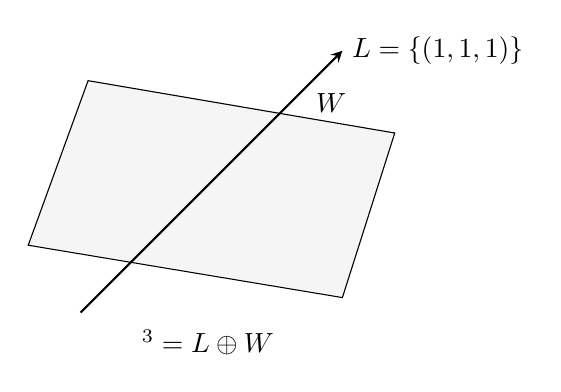
\begin{tikzpicture}[scale=0.95,>=stealth]
\draw[fill=gray!8] (-2.4,-0.8)--(1.8,-1.5)--(2.5,0.7)--(-1.6,1.4)--cycle;
\node at (1.65,1.1) {\(W\)};

\draw[->,thick] (-1.7,-1.7)--(1.8,1.8);
\node[right] at (1.8,1.8) {\(L=\Span\{(1,1,1)\}\)};

\node at (0,-2.1) {\(\R^3=L\oplus W\)};
\end{tikzpicture}
\end{center}

%%%%%%%%%%%%%%%%%%%%%%%%%%%%%%%%%%%%%%%%%%%%%%%%%%%%%%%%%%%%
\subsection{Character Table of \(S_3\)}
\label{subsec:s3-character-table}
%%%%%%%%%%%%%%%%%%%%%%%%%%%%%%%%%%%%%%%%%%%%%%%%%%%%%%%%%%%%

The irreducible character table is

\begin{center}
\begin{tabular}{c|ccc}
\toprule
 & \(e\) & \((12)\) & \((123)\)\\
\midrule
Class size & \(1\) & \(3\) & \(2\)\\
\midrule
\(\chi_{\mathrm{triv}}\) & \(1\) & \(1\) & \(1\)\\
\(\chi_{\mathrm{sgn}}\) & \(1\) & \(-1\) & \(1\)\\
\(\chi_{\mathrm{std}}\) & \(2\) & \(0\) & \(-1\)\\
\bottomrule
\end{tabular}
\end{center}

The first column confirms the dimensions:

\[ 1,\qquad1,\qquad2. \]

Their squared dimensions satisfy

\[ 1^2+1^2+2^2=6=|S_3|. \]

%%%%%%%%%%%%%%%%%%%%%%%%%%%%%%%%%%%%%%%%%%%%%%%%%%%%%%%%%%%%
\subsection{Worked Example: Testing the Standard Character}
\label{subsec:worked-standard-character}
%%%%%%%%%%%%%%%%%%%%%%%%%%%%%%%%%%%%%%%%%%%%%%%%%%%%%%%%%%%%

\begin{workedexamplebox}{Testing Irreducibility with Characters}

For \(S_3\), let

\[ \chi=(2,0,-1) \]

on conjugacy classes of sizes

\[ 1,\qquad3,\qquad2. \]

Compute \(\inner{\chi,\chi}\).

\begin{tabularx}{\textwidth}{@{}>{\raggedright\arraybackslash}p{0.42\textwidth}X@{}}
Use the class form of the inner product. &
\(\displaystyle
\inner{\chi,\chi}
=\frac16\left(1|2|^2+3|0|^2+2|-1|^2\right)\)\\
Evaluate. &
\(\displaystyle
\inner{\chi,\chi}
=\frac16(4+0+2)\)\\
Simplify. & \(\displaystyle \inner{\chi,\chi}=1\)\\
Apply the irreducibility criterion. & The character is irreducible.
\end{tabularx}

\begin{answerbox}
\[ \boxed{\inner{\chi,\chi}=1,\qquad\chi\text{ is irreducible}.} \]
\end{answerbox}
\end{workedexamplebox}

%%%%%%%%%%%%%%%%%%%%%%%%%%%%%%%%%%%%%%%%%%%%%%%%%%%%%%%%%%%%
\subsection{Tensor Products of Representations}
\label{subsec:tensor-product-representations}
%%%%%%%%%%%%%%%%%%%%%%%%%%%%%%%%%%%%%%%%%%%%%%%%%%%%%%%%%%%%

Suppose \(V\) and \(W\) are representations of \(G\).

Their tensor product

\[ V\otimes W \]

becomes a representation by defining

\[ g\cdot(v\otimes w)=(g\cdot v)\otimes(g\cdot w). \]

Equivalently,

\[ (\rho_V\otimes\rho_W)(g)
=\rho_V(g)\otimes\rho_W(g). \]

The symbol

\[ \otimes \]

is the tensor-product symbol and is read ``tensor.''

%%%%%%%%%%%%%%%%%%%%%%%%%%%%%%%%%%%%%%%%%%%%%%%%%%%%%%%%%%%%
\subsection{Character of a Tensor Product}
\label{subsec:character-tensor-product}
%%%%%%%%%%%%%%%%%%%%%%%%%%%%%%%%%%%%%%%%%%%%%%%%%%%%%%%%%%%%

A fundamental trace identity gives

\[ \tr(A\otimes B)=\tr(A)\tr(B). \]

Therefore,

\[ \boxed{\chi_{V\otimes W}(g)=\chi_V(g)\chi_W(g).} \]

Thus direct sums correspond to addition of characters, while tensor products
correspond to multiplication:

\[ \chi_{V\oplus W}=\chi_V+\chi_W, \]

\[ \chi_{V\otimes W}=\chi_V\chi_W. \]

%%%%%%%%%%%%%%%%%%%%%%%%%%%%%%%%%%%%%%%%%%%%%%%%%%%%%%%%%%%%
\subsection{Dual Representations}
\label{subsec:dual-representations}
%%%%%%%%%%%%%%%%%%%%%%%%%%%%%%%%%%%%%%%%%%%%%%%%%%%%%%%%%%%%

Let

\[ V^*=\Hom_F(V,F) \]

be the dual vector space.

The dual representation is defined by

\[ (g\cdot\varphi)(v)=\varphi(g^{-1}\cdot v). \]

Here \(\varphi\in V^*\).

In matrix form,

\[ \rho_{V^*}(g)=\rho_V(g^{-1})^{\mathsf T}. \]

The superscript

\[ \mathsf T \]

denotes transpose and is read ``transpose.''

%%%%%%%%%%%%%%%%%%%%%%%%%%%%%%%%%%%%%%%%%%%%%%%%%%%%%%%%%%%%
\subsection{Character of the Dual}
\label{subsec:character-dual}
%%%%%%%%%%%%%%%%%%%%%%%%%%%%%%%%%%%%%%%%%%%%%%%%%%%%%%%%%%%%

For a finite-dimensional complex representation,

\[ \chi_{V^*}(g)=\chi_V(g^{-1}). \]

For unitary representations of finite groups,

\[ \chi_V(g^{-1})=\overline{\chi_V(g)}. \]

Therefore,

\[ \chi_{V^*}(g)=\overline{\chi_V(g)}. \]

%%%%%%%%%%%%%%%%%%%%%%%%%%%%%%%%%%%%%%%%%%%%%%%%%%%%%%%%%%%%
\subsection{Quotient Representations}
\label{subsec:quotient-representations}
%%%%%%%%%%%%%%%%%%%%%%%%%%%%%%%%%%%%%%%%%%%%%%%%%%%%%%%%%%%%

Suppose \(W\subseteq V\) is an invariant subspace.

Then the quotient vector space

\[ V/W \]

inherits a representation:

\[ g\cdot(v+W)=g\cdot v+W. \]

This is well defined precisely because \(W\) is invariant.

Thus invariant subspaces produce both:

\[ W \]

as a subrepresentation and

\[ V/W \]

as a quotient representation.

%%%%%%%%%%%%%%%%%%%%%%%%%%%%%%%%%%%%%%%%%%%%%%%%%%%%%%%%%%%%
\subsection{Exact Sequences of Representations}
\label{subsec:exact-sequences-representations}
%%%%%%%%%%%%%%%%%%%%%%%%%%%%%%%%%%%%%%%%%%%%%%%%%%%%%%%%%%%%

A subrepresentation \(W\subseteq V\) gives a short exact sequence

\[ 0\longrightarrow W\longrightarrow V\longrightarrow V/W\longrightarrow0. \]

This notation will become central in homological algebra.

When the sequence splits,

\[ V\cong W\oplus V/W. \]

Maschke's theorem implies that such sequences split for finite-dimensional
representations of finite groups when the characteristic of the field does
not divide the group order.

%%%%%%%%%%%%%%%%%%%%%%%%%%%%%%%%%%%%%%%%%%%%%%%%%%%%%%%%%%%%
\subsection{Unitary Representations}
\label{subsec:unitary-representations}
%%%%%%%%%%%%%%%%%%%%%%%%%%%%%%%%%%%%%%%%%%%%%%%%%%%%%%%%%%%%

A complex representation is \emph{unitary} if each group element acts by a
unitary transformation.

Thus

\[ \rho(g)^*\rho(g)=I. \]

The symbol

\[ A^* \]

denotes the conjugate transpose of \(A\) and is read ``\(A\) star.''

For finite groups over \(\C\), every finite-dimensional representation is
equivalent to a unitary representation.

Again, averaging provides the key idea: average an inner product over the
group to produce a \(G\)-invariant inner product.

%%%%%%%%%%%%%%%%%%%%%%%%%%%%%%%%%%%%%%%%%%%%%%%%%%%%%%%%%%%%
\subsection{Averaging an Inner Product}
\label{subsec:averaging-inner-product}
%%%%%%%%%%%%%%%%%%%%%%%%%%%%%%%%%%%%%%%%%%%%%%%%%%%%%%%%%%%%

Begin with any Hermitian inner product

\[ \inner{v,w}_0. \]

Define

\[ \inner{v,w}_G
=\frac{1}{|G|}\sum_{g\in G}
\inner{\rho(g)v,\rho(g)w}_0. \]

Then

\[ \inner{\rho(h)v,\rho(h)w}_G=\inner{v,w}_G \]

for every \(h\in G\).

Thus the representation becomes unitary relative to this averaged inner
product.

%%%%%%%%%%%%%%%%%%%%%%%%%%%%%%%%%%%%%%%%%%%%%%%%%%%%%%%%%%%%
\subsection{Restriction of Representations}
\label{subsec:restriction-representations}
%%%%%%%%%%%%%%%%%%%%%%%%%%%%%%%%%%%%%%%%%%%%%%%%%%%%%%%%%%%%

Let

\[ H\leq G. \]

A representation

\[ \rho:G\to GL(V) \]

can be restricted to \(H\):

\[ \rho|_H:H\to GL(V). \]

This is called the \emph{restriction} of the representation from \(G\) to
\(H\).

One often writes

\[ \operatorname{Res}^G_H V. \]

The notation is read ``the restriction from \(G\) to \(H\) of \(V\).''

An irreducible representation of \(G\) may become reducible when restricted
to a subgroup.

%%%%%%%%%%%%%%%%%%%%%%%%%%%%%%%%%%%%%%%%%%%%%%%%%%%%%%%%%%%%
\subsection{Induced Representations: A Preview}
\label{subsec:induced-representations}
%%%%%%%%%%%%%%%%%%%%%%%%%%%%%%%%%%%%%%%%%%%%%%%%%%%%%%%%%%%%

There is also a construction moving in the opposite direction.

Starting with a representation \(W\) of a subgroup

\[ H\leq G, \]

one can construct a representation of \(G\) called the \emph{induced
representation}.

It is denoted

\[ \operatorname{Ind}_H^G W. \]

This is read ``the representation induced from \(H\) to \(G\) by \(W\).''

Restriction moves representations downward to subgroups; induction moves
them upward to larger groups.

\begin{center}
\begin{tikzcd}[column sep=large]
G\text{-representations}
\arrow[r,shift left=1.2ex,"\operatorname{Res}^G_H"]
&
H\text{-representations}
\arrow[l,shift left=1.2ex,"\operatorname{Ind}_H^G"]
\end{tikzcd}
\end{center}

%%%%%%%%%%%%%%%%%%%%%%%%%%%%%%%%%%%%%%%%%%%%%%%%%%%%%%%%%%%%
\subsection{Frobenius Reciprocity: A Preview}
\label{subsec:frobenius-reciprocity-preview}
%%%%%%%%%%%%%%%%%%%%%%%%%%%%%%%%%%%%%%%%%%%%%%%%%%%%%%%%%%%%

Induction and restriction are related by Frobenius reciprocity.

In one common form,

\[ \Hom_G(\operatorname{Ind}_H^G W,V)
\cong
\Hom_H(W,\operatorname{Res}_H^G V). \]

This theorem expresses a deep compatibility between representations of a
group and representations of its subgroups.

A full treatment requires a more detailed development of induced modules and
is deferred to advanced representation theory.

%%%%%%%%%%%%%%%%%%%%%%%%%%%%%%%%%%%%%%%%%%%%%%%%%%%%%%%%%%%%
\subsection{Representations of Algebras}
\label{subsec:representations-of-algebras}
%%%%%%%%%%%%%%%%%%%%%%%%%%%%%%%%%%%%%%%%%%%%%%%%%%%%%%%%%%%%

Representation theory is not limited to groups.

Let \(A\) be an \(F\)-algebra.

A representation of \(A\) on \(V\) is an algebra homomorphism

\[ \rho:A\to\End_F(V). \]

Thus elements of \(A\) act as linear operators.

Equivalently, \(V\) becomes an \(A\)-module.

This perspective includes representations of:

\begin{itemize}
    \item group algebras;
    \item associative algebras;
    \item Lie algebras;
    \item operator algebras;
    \item quiver algebras.
\end{itemize}

%%%%%%%%%%%%%%%%%%%%%%%%%%%%%%%%%%%%%%%%%%%%%%%%%%%%%%%%%%%%
\subsection{Representations of Lie Groups and Lie Algebras}
\label{subsec:representation-lie-preview}
%%%%%%%%%%%%%%%%%%%%%%%%%%%%%%%%%%%%%%%%%%%%%%%%%%%%%%%%%%%%

Representation theory becomes especially important for Lie groups and Lie
algebras.

A Lie group representation typically has the form

\[ \rho:G\to GL(V), \]

with additional smoothness conditions.

A Lie algebra representation has the form

\[ \rho:\mathfrak g\to\mathfrak{gl}(V), \]

where the fraktur symbol

\[ \mathfrak g \]

is read ``fraktur \(g\)'' and commonly denotes a Lie algebra.

The notation

\[ \mathfrak{gl}(V) \]

denotes the Lie algebra of linear endomorphisms of \(V\).

These structures are developed canonically in
\cref{sec:lie-groups-lie-algebras}.

%%%%%%%%%%%%%%%%%%%%%%%%%%%%%%%%%%%%%%%%%%%%%%%%%%%%%%%%%%%%
\subsection{Symmetry Through Representations}
\label{subsec:symmetry-through-representations}
%%%%%%%%%%%%%%%%%%%%%%%%%%%%%%%%%%%%%%%%%%%%%%%%%%%%%%%%%%%%

Representation theory is fundamentally a mathematical theory of symmetry.

A symmetry group may be abstract, but a representation describes how those
symmetries act on an actual mathematical space.

\begin{center}
\begin{tikzpicture}[
    node distance=12mm and 18mm,
    box/.style={draw,rounded corners,align=center,inner sep=5pt},
    >=stealth
]
\node[box] (sym) {Abstract symmetry\\group \(G\)};
\node[box,below left=of sym] (geo) {Geometric\\space};
\node[box,below=of sym] (vec) {Vector\\space};
\node[box,below right=of sym] (func) {Function\\space};

\node[box,below=24mm of sym] (rep) {Representation theory};

\draw[->,thick] (sym)--(geo);
\draw[->,thick] (sym)--(vec);
\draw[->,thick] (sym)--(func);
\draw[->,thick] (geo)--(rep);
\draw[->,thick] (vec)--(rep);
\draw[->,thick] (func)--(rep);
\end{tikzpicture}
\end{center}

%%%%%%%%%%%%%%%%%%%%%%%%%%%%%%%%%%%%%%%%%%%%%%%%%%%%%%%%%%%%
\subsection{Representation Theory and Geometry}
\label{subsec:representation-geometry}
%%%%%%%%%%%%%%%%%%%%%%%%%%%%%%%%%%%%%%%%%%%%%%%%%%%%%%%%%%%%

Geometric objects often possess symmetry groups.

Representations describe how those symmetries act on:

\begin{itemize}
    \item tangent spaces;
    \item coordinate spaces;
    \item polynomial spaces;
    \item differential forms;
    \item spaces of functions.
\end{itemize}

For example, rotations of a polygon act naturally on the plane, producing a
two-dimensional representation of a dihedral group.

%%%%%%%%%%%%%%%%%%%%%%%%%%%%%%%%%%%%%%%%%%%%%%%%%%%%%%%%%%%%
\subsection{Representation Theory and Differential Equations}
\label{subsec:representation-differential-equations}
%%%%%%%%%%%%%%%%%%%%%%%%%%%%%%%%%%%%%%%%%%%%%%%%%%%%%%%%%%%%

Symmetries of differential equations can act on their spaces of solutions.

Representation theory can then decompose a complicated solution space into
simpler invariant pieces.

This philosophy appears in:

\begin{itemize}
    \item Fourier analysis;
    \item spherical harmonics;
    \item partial differential equations;
    \item spectral theory;
    \item mathematical physics.
\end{itemize}

%%%%%%%%%%%%%%%%%%%%%%%%%%%%%%%%%%%%%%%%%%%%%%%%%%%%%%%%%%%%
\subsection{Representation Theory and Quantum Mechanics}
\label{subsec:representation-quantum}
%%%%%%%%%%%%%%%%%%%%%%%%%%%%%%%%%%%%%%%%%%%%%%%%%%%%%%%%%%%%

Quantum mechanics makes extensive use of representations of symmetry groups.

Physical states form vector spaces, while symmetries act through linear or
unitary transformations.

Angular momentum, spin, rotational symmetry, and particle classifications
are deeply connected to representations of groups and Lie algebras.

The mathematical principle is:

\[ \text{symmetry}\longrightarrow\text{linear operators}. \]

%%%%%%%%%%%%%%%%%%%%%%%%%%%%%%%%%%%%%%%%%%%%%%%%%%%%%%%%%%%%
\subsection{Representation Theory and Fourier Analysis}
\label{subsec:representation-fourier}
%%%%%%%%%%%%%%%%%%%%%%%%%%%%%%%%%%%%%%%%%%%%%%%%%%%%%%%%%%%%

Classical Fourier analysis can be interpreted using representations of
abelian groups.

For a finite cyclic group, irreducible characters are roots of unity.

For continuous abelian groups, analogous characters lead to exponential
functions such as

\[ e^{2\pi i\xi x}. \]

Thus Fourier decomposition can be viewed as decomposition into irreducible
representations of an abelian symmetry group.

This connection is developed further in the analysis branch.

%%%%%%%%%%%%%%%%%%%%%%%%%%%%%%%%%%%%%%%%%%%%%%%%%%%%%%%%%%%%
\subsection{A Structural Hierarchy}
\label{subsec:representation-structural-hierarchy}
%%%%%%%%%%%%%%%%%%%%%%%%%%%%%%%%%%%%%%%%%%%%%%%%%%%%%%%%%%%%

Representation theory can be organized around decomposition:

\begin{center}
\begin{tikzpicture}[
    node distance=10mm and 13mm,
    box/.style={draw,rounded corners,align=center,inner sep=5pt,font=\small},
    >=stealth
]
\node[box] (rep) {Representation \(V\)};
\node[box,below=of rep] (inv) {Invariant subspaces};
\node[box,below left=of inv] (red) {Reducible};
\node[box,below right=of inv] (irr) {Irreducible};
\node[box,below=of red] (direct) {Direct-sum\\decomposition};
\node[box,below=of direct] (chars) {Characters};
\node[box,below=of irr] (blocks) {Basic building\\blocks};

\draw[->] (rep)--(inv);
\draw[->] (inv)--(red);
\draw[->] (inv)--(irr);
\draw[->] (red)--(direct);
\draw[->] (direct)--(chars);
\draw[->] (irr)--(blocks);
\draw[->] (chars)--(blocks);
\end{tikzpicture}
\end{center}

%%%%%%%%%%%%%%%%%%%%%%%%%%%%%%%%%%%%%%%%%%%%%%%%%%%%%%%%%%%%
\subsection{Worked Example: A Representation of \(C_4\)}
\label{subsec:worked-c4-representation}
%%%%%%%%%%%%%%%%%%%%%%%%%%%%%%%%%%%%%%%%%%%%%%%%%%%%%%%%%%%%

\begin{workedexamplebox}{Representing \(C_4\) by Rotations}

Let

\[ C_4=\langle g:g^4=e\rangle. \]

Represent \(g\) as rotation through \(90^\circ\).

\begin{tabularx}{\textwidth}{@{}>{\raggedright\arraybackslash}p{0.42\textwidth}X@{}}
Use the rotation matrix. &
\(\displaystyle
\rho(g)=
\begin{pmatrix}
0&-1\\
1&0
\end{pmatrix}\)\\
Square the matrix. &
\(\displaystyle
\rho(g)^2=
\begin{pmatrix}
-1&0\\
0&-1
\end{pmatrix}\)\\
Raise to the fourth power. &
\(\displaystyle \rho(g)^4=I_2\)\\
Compare with the group relation. & \(g^4=e\) is preserved.
\end{tabularx}

\begin{answerbox}
\[ \boxed{\rho(g)=\begin{pmatrix}0&-1\\1&0\end{pmatrix},\qquad
\rho(g)^4=I_2.} \]
\end{answerbox}
\end{workedexamplebox}

%%%%%%%%%%%%%%%%%%%%%%%%%%%%%%%%%%%%%%%%%%%%%%%%%%%%%%%%%%%%
\subsection{Worked Example: Kernel and Faithfulness}
\label{subsec:worked-faithful-representation}
%%%%%%%%%%%%%%%%%%%%%%%%%%%%%%%%%%%%%%%%%%%%%%%%%%%%%%%%%%%%

\begin{workedexamplebox}{Testing Faithfulness}

Let

\[ C_4=\langle g\rangle \]

and define a one-dimensional complex representation by

\[ \rho(g)=i. \]

Determine whether \(\rho\) is faithful.

\begin{tabularx}{\textwidth}{@{}>{\raggedright\arraybackslash}p{0.42\textwidth}X@{}}
Compute the images of powers. &
\(\rho(e)=1,\ \rho(g)=i,\ \rho(g^2)=-1,\ \rho(g^3)=-i\)\\
Identify elements mapping to \(1\). & Only \(e\) maps to \(1\).\\
Find the kernel. & \(\Ker(\rho)=\{e\}\)\\
Apply the definition. & The representation is faithful.
\end{tabularx}

\begin{answerbox}
\[ \boxed{\rho\text{ is faithful}.} \]
\end{answerbox}
\end{workedexamplebox}

%%%%%%%%%%%%%%%%%%%%%%%%%%%%%%%%%%%%%%%%%%%%%%%%%%%%%%%%%%%%
\subsection{Worked Example: Character Decomposition}
\label{subsec:worked-character-decomposition}
%%%%%%%%%%%%%%%%%%%%%%%%%%%%%%%%%%%%%%%%%%%%%%%%%%%%%%%%%%%%

\begin{workedexamplebox}{Finding Multiplicity from a Character}

Suppose \(\chi\) is a character of a finite group and \(\psi\) is an
irreducible character. Assume

\[ \inner{\chi,\psi}=3. \]

Determine the multiplicity of the irreducible representation corresponding
to \(\psi\).

\begin{tabularx}{\textwidth}{@{}>{\raggedright\arraybackslash}p{0.42\textwidth}X@{}}
Use the multiplicity formula. & \(m_\psi=\inner{\chi,\psi}\)\\
Substitute the given value. & \(m_\psi=3\)
\end{tabularx}

\begin{answerbox}
\[ \boxed{\psi\text{ occurs with multiplicity }3.} \]
\end{answerbox}
\end{workedexamplebox}

%%%%%%%%%%%%%%%%%%%%%%%%%%%%%%%%%%%%%%%%%%%%%%%%%%%%%%%%%%%%
\subsection{Common Errors}
\label{subsec:representation-common-errors}
%%%%%%%%%%%%%%%%%%%%%%%%%%%%%%%%%%%%%%%%%%%%%%%%%%%%%%%%%%%%

\subsubsection{Assigning Matrices Without Checking the Group Law}

A collection of matrices does not define a representation unless

\[ \rho(gh)=\rho(g)\rho(h). \]

For a group given by generators and relations, the matrices must satisfy the
same relations.

%%%%%%%%%%%%%%%%%%%%%%%%%%%%%%%%%%%%%%%%%%%%%%%%%%%%%%%%%%%%
\subsubsection{Confusing a Representation with Its Matrix Form}

A representation acts on a vector space.

Matrices appear only after choosing a basis.

Different matrices may therefore describe equivalent representations.

%%%%%%%%%%%%%%%%%%%%%%%%%%%%%%%%%%%%%%%%%%%%%%%%%%%%%%%%%%%%
\subsubsection{Confusing Faithful with Irreducible}

Faithfulness concerns the kernel:

\[ \Ker(\rho)=\{e\}. \]

Irreducibility concerns invariant subspaces.

Neither condition implies the other in general.

%%%%%%%%%%%%%%%%%%%%%%%%%%%%%%%%%%%%%%%%%%%%%%%%%%%%%%%%%%%%
\subsubsection{Checking Invariance Under Only One Element}

A subspace \(W\) is \(G\)-invariant only if

\[ \rho(g)W\subseteq W \]

for every \(g\in G\).

If the group is generated by a set \(S\), however, it is enough to check the
generators.

%%%%%%%%%%%%%%%%%%%%%%%%%%%%%%%%%%%%%%%%%%%%%%%%%%%%%%%%%%%%
\subsubsection{Assuming Reducible Means Already Decomposed}

A reducible representation contains a nontrivial invariant subspace.

That alone does not automatically give a direct-sum decomposition over every
field and in every characteristic.

Maschke's theorem provides such decompositions under specific hypotheses.

%%%%%%%%%%%%%%%%%%%%%%%%%%%%%%%%%%%%%%%%%%%%%%%%%%%%%%%%%%%%
\subsubsection{Ignoring the Characteristic}

For a finite group \(G\), Maschke's theorem requires

\[ \operatorname{char}(F)\nmid|G|. \]

If the characteristic divides the group order, representations may fail to
be completely reducible.

%%%%%%%%%%%%%%%%%%%%%%%%%%%%%%%%%%%%%%%%%%%%%%%%%%%%%%%%%%%%
\subsubsection{Confusing Characters with Representations}

A character is a function obtained from a representation:

\[ \chi_\rho(g)=\tr(\rho(g)). \]

It summarizes important information but is not itself the original matrix
representation.

%%%%%%%%%%%%%%%%%%%%%%%%%%%%%%%%%%%%%%%%%%%%%%%%%%%%%%%%%%%%
\subsubsection{Forgetting Conjugacy Classes}

Characters are constant on conjugacy classes.

A character table therefore has columns indexed by conjugacy classes, not
necessarily by individual elements.

%%%%%%%%%%%%%%%%%%%%%%%%%%%%%%%%%%%%%%%%%%%%%%%%%%%%%%%%%%%%
\subsubsection{Forgetting Class Sizes in Inner Products}

When computing a character inner product class by class, each character
value must be multiplied by the size of its conjugacy class.

%%%%%%%%%%%%%%%%%%%%%%%%%%%%%%%%%%%%%%%%%%%%%%%%%%%%%%%%%%%%
\subsection{Applications}
\label{subsec:representation-applications}
%%%%%%%%%%%%%%%%%%%%%%%%%%%%%%%%%%%%%%%%%%%%%%%%%%%%%%%%%%%%

\begin{applicationbox}
\textbf{Group Theory.}
Representations turn abstract groups into matrix groups and reveal structural
information through linear algebra.

\medskip

\textbf{Noncommutative Algebra.}
Representations of groups correspond to modules over group algebras, linking
representation theory directly with module and ring theory.

\medskip

\textbf{Geometry.}
Symmetry groups act on geometric spaces, tangent spaces, coordinate spaces,
and spaces of functions.

\medskip

\textbf{Number Theory.}
Representations of finite groups, Galois groups, and arithmetic groups play
major roles in modern number theory.

\medskip

\textbf{Fourier Analysis.}
Characters of abelian groups generalize the exponential functions underlying
Fourier series and Fourier transforms.

\medskip

\textbf{Differential Equations.}
Symmetry representations can decompose solution spaces into simpler
invariant components.

\medskip

\textbf{Quantum Mechanics.}
Physical symmetries are represented by linear or unitary operators on state
spaces.

\medskip

\textbf{Particle Physics.}
Representations of Lie groups and Lie algebras classify many symmetry types
and particle states.

\medskip

\textbf{Chemistry.}
Molecular symmetry and spectroscopy use representations and character tables
to classify vibrational and orbital behavior.
\end{applicationbox}

%%%%%%%%%%%%%%%%%%%%%%%%%%%%%%%%%%%%%%%%%%%%%%%%%%%%%%%%%%%%
\subsection{Exercises}
\label{subsec:representation-exercises}
%%%%%%%%%%%%%%%%%%%%%%%%%%%%%%%%%%%%%%%%%%%%%%%%%%%%%%%%%%%%

\begin{exercise}[1]
State the definition of a representation
\[ \rho:G\to GL(V). \]
\end{exercise}

\begin{exercise}[1]
Show that every representation satisfies
\[ \rho(e)=I_V. \]
\end{exercise}

\begin{exercise}[1]
Show that
\[ \rho(g^{-1})=\rho(g)^{-1}. \]
\end{exercise}

\begin{exercise}[1]
Define the trivial representation of a group \(G\).
\end{exercise}

\begin{exercise}[1]
What is the degree of a representation on \(F^5\)?
\end{exercise}

\begin{exercise}[2]
Let
\[ C_3=\langle g\rangle. \]
Show that
\[ \rho(g)=e^{2\pi i/3} \]
defines a one-dimensional complex representation.
\end{exercise}

\begin{exercise}[2]
Let
\[ C_4=\langle g\rangle. \]
Determine whether
\[ \rho(g)=
\begin{pmatrix}
0&-1\\
1&0
\end{pmatrix}
\]
defines a representation of \(C_4\).
\end{exercise}

\begin{exercise}[1]
Define the kernel of a representation.
\end{exercise}

\begin{exercise}[1]
Define a faithful representation.
\end{exercise}

\begin{exercise}[2]
Prove that a representation is faithful if and only if it is injective.
\end{exercise}

\begin{exercise}[2]
Show that the left regular representation is faithful.
\end{exercise}

\begin{exercise}[1]
Define a \(G\)-invariant subspace.
\end{exercise}

\begin{exercise}[2]
Show that
\[ \Span\{(1,1,\ldots,1)\} \]
is invariant under every permutation representation on \(F^n\).
\end{exercise}

\begin{exercise}[1]
Distinguish reducible and irreducible representations.
\end{exercise}

\begin{exercise}[2]
Show that every one-dimensional nonzero representation is irreducible.
\end{exercise}

\begin{exercise}[1]
Define the direct sum
\[ V\oplus W \]
of two representations.
\end{exercise}

\begin{exercise}[2]
Verify that
\[ \rho_1\oplus\rho_2 \]
satisfies the representation homomorphism condition.
\end{exercise}

\begin{exercise}[1]
State Maschke's theorem.
\end{exercise}

\begin{exercise}[2]
Explain why the condition
\[ \operatorname{char}(F)\nmid|G| \]
is necessary for the averaging argument in Maschke's theorem.
\end{exercise}

\begin{exercise}[2]
Let \(G\) be a finite group acting on a complex vector space. Explain how
averaging can produce a \(G\)-invariant inner product.
\end{exercise}

\begin{exercise}[1]
Define an intertwining map.
\end{exercise}

\begin{exercise}[2]
Show that the kernel of an intertwining map is invariant.
\end{exercise}

\begin{exercise}[2]
Show that the image of an intertwining map is invariant.
\end{exercise}

\begin{exercise}[2]
Use the previous two exercises to prove Schur's lemma.
\end{exercise}

\begin{exercise}[1]
Define equivalent representations.
\end{exercise}

\begin{exercise}[2]
Show that a change of basis produces an equivalent matrix representation.
\end{exercise}

\begin{exercise}[1]
Define the character of a representation.
\end{exercise}

\begin{exercise}[1]
Show that
\[ \chi(e)=\dim(V). \]
\end{exercise}

\begin{exercise}[2]
Prove that equivalent representations have the same character.
\end{exercise}

\begin{exercise}[2]
Prove that characters are constant on conjugacy classes.
\end{exercise}

\begin{exercise}[1]
Compute the character of
\[ A=\begin{pmatrix}2&0\\0&-1\end{pmatrix}. \]
\end{exercise}

\begin{exercise}[1]
Compute the character of a plane rotation through angle \(\theta\).
\end{exercise}

\begin{exercise}[2]
Prove that
\[ \chi_{V\oplus W}=\chi_V+\chi_W. \]
\end{exercise}

\begin{exercise}[2]
Prove that
\[ \chi_{V\otimes W}=\chi_V\chi_W. \]
\end{exercise}

\begin{exercise}[1]
Define the inner product of two complex characters of a finite group.
\end{exercise}

\begin{exercise}[2]
For the \(S_3\) character
\[ \chi=(2,0,-1), \]
verify that
\[ \inner{\chi,\chi}=1. \]
\end{exercise}

\begin{exercise}[2]
Using the \(S_3\) character table, verify that
\[ \inner{\chi_{\mathrm{triv}},\chi_{\mathrm{sgn}}}=0. \]
\end{exercise}

\begin{exercise}[2]
Using the \(S_3\) character table, verify that
\[ \inner{\chi_{\mathrm{std}},\chi_{\mathrm{triv}}}=0. \]
\end{exercise}

\begin{exercise}[1]
State the sum of squares formula for irreducible representation dimensions.
\end{exercise}

\begin{exercise}[2]
Suppose a group has order \(8\) and four one-dimensional irreducible
representations. If there is exactly one additional irreducible
representation, determine its dimension.
\end{exercise}

\begin{exercise}[2]
Suppose a finite group has irreducible representation dimensions
\[ 1,1,2,3. \]
Determine the order of the group.
\end{exercise}

\begin{exercise}[2]
Explain why every irreducible complex representation of a finite abelian
group is one-dimensional.
\end{exercise}

\begin{exercise}[2]
Determine the character of the regular representation of a group of order
\(10\).
\end{exercise}

\begin{exercise}[2]
If an irreducible representation has dimension \(4\), how many copies of it
occur in the regular representation?
\end{exercise}

\begin{exercise}[1]
Define the dual representation \(V^*\).
\end{exercise}

\begin{exercise}[2]
Show that
\[ \rho_{V^*}(g)=\rho_V(g^{-1})^{\mathsf T}. \]
\end{exercise}

\begin{exercise}[1]
Define a quotient representation.
\end{exercise}

\begin{exercise}[2]
Explain why invariance of \(W\) is necessary for the action on
\[ V/W \]
to be well defined.
\end{exercise}

\begin{exercise}[1]
Define the restriction
\[ \operatorname{Res}_H^G V. \]
\end{exercise}

\begin{exercise}[2]
Give an example of an irreducible representation that becomes reducible when
restricted to a subgroup.
\end{exercise}

\begin{exercise}[1]
What is meant by an induced representation?
\end{exercise}

\begin{exercise}[2]
Explain conceptually how restriction and induction move in opposite
directions.
\end{exercise}

\begin{exercise}[2]
Show explicitly that representations of \(G\) over \(F\) correspond to
\(F[G]\)-modules.
\end{exercise}

\begin{exercise}[3]
For the permutation representation of \(S_3\) on \(\R^3\), prove that
\[ \R^3=\Span\{(1,1,1)\}\oplus
\{(x,y,z):x+y+z=0\}. \]
Show that both summands are invariant.
\end{exercise}

\begin{exercise}[3]
Using the character table of \(S_3\), decompose the three-dimensional
permutation representation into irreducible representations.
\end{exercise}

%%%%%%%%%%%%%%%%%%%%%%%%%%%%%%%%%%%%%%%%%%%%%%%%%%%%%%%%%%%%
\subsection{Section Connections}
\label{subsec:representation-theory-connections}
%%%%%%%%%%%%%%%%%%%%%%%%%%%%%%%%%%%%%%%%%%%%%%%%%%%%%%%%%%%%

\chapterconnection{
Representation theory converts abstract algebraic structure into linear
transformations. Group representations therefore connect group theory with
linear algebra, while the equivalence between group representations and
modules over group algebras connects the subject directly with module theory
and noncommutative algebra. Irreducible representations serve as basic
building blocks, Maschke's theorem explains when complete decomposition is
possible, and Schur's lemma describes maps between irreducible pieces.
Characters compress matrix information into class functions and provide
powerful tools for testing irreducibility and determining multiplicities.
Tensor products, duals, restrictions, and induced representations provide
new ways to construct representations. These ideas prepare for
\cref{sec:lie-groups-lie-algebras}, while character theory connects naturally
with Fourier analysis, geometry, number theory, differential equations, and
mathematical physics.
}

%%%%%%%%%%%%%%%%%%%%%%%%%%%%%%%%%%%%%%%%%%%%%%%%%%%%%%%%%%%%
% SECTION SOURCE TRACKING
%%%%%%%%%%%%%%%%%%%%%%%%%%%%%%%%%%%%%%%%%%%%%%%%%%%%%%%%%%%%

%------------------------------------------------------------
% 1.11 Representation Theory
%------------------------------------------------------------
%
% Sources:
%   - William Fulton and Joe Harris,
%     Representation Theory: A First Course.
%     Key: fultonharris1991representation
%
% Used for:
%   - representation and irreducibility framework;
%   - invariant subspaces and decomposition;
%   - intertwining maps and equivalent representations;
%   - Schur's lemma;
%   - characters and character-theoretic structure;
%   - direct sums, tensor products, and dual representations;
%   - structural connections with finite-group representations.
%
% Notes:
%   - Group foundations are treated canonically in Section 1.4.
%   - Module foundations are treated canonically in Section 1.8.
%   - Group algebras and semisimple-ring background are introduced in
%     Section 1.10.
%   - Lie group and Lie algebra representation theory is introduced only as
%     a bridge to Section 1.12.
%   - Induced representations and Frobenius reciprocity are presented as
%     introductory previews rather than complete advanced treatments.
%   - Applications to physics, chemistry, Fourier analysis, and differential
%     equations are included as connections rather than replacements for
%     their canonical treatments elsewhere in the text.
%   - Visualizations and pedagogical organization are independently
%     developed for this text.
%
\nocite{fultonharris1991representation}